\section{Background}
\subsection{Recommendation Systems}
Recommendation systems predict the preferences of users in regard to new items or objects, in the form of a ranking of items or objects, rating items or objects, or classifying items or objects \cite{DBLP:journals/corr/ZhangYS17aa}. There exist a wide variety of established strategies to learn prediction models for recommendation systems, generally fitting into three categories: collaborative filtering, content based, or hybrid systems. Collaborative filtering based recommendation system models learn based on user - item/object interaction, while content based recommendation system models learn based on intrinsic user and item/object characteristics. Hybrid recommendation system models learn based on a combination of the two approaches.  
\subsection{Deep Learning}
Deep learning is a subset of machine learning wherein models learned contain multiple, often heiarchical, abstractions or representations. While there are many approaches to deep learning, in this paper we employ deep feedforward neural networks - feed forward neural networks with one or more hidden layers. A general interpretation of the hidden layers in a deep feedforward neural network is that each layer learns a slightly more complex representation of the data than the layer before it.
\subsection{Embedding Layers}
Embedding layers encode information about a set of objects and the relationships between those objects in a latent space - generally with fewer dimensions than the original space representing the objects \cite{DBLP:journals/corr/abs-1301-3781}. For example, given a corpus of text with a large vocabulary \textit{V}, it may be desireable to represent $\textit{v}\in\textit{V}$ such that $\mid\textit{rep(v)}\mid=\textit{k}$, where $\textit{k}\ll\mid\textit{V}\mid$ and that if \textit{v}, $\textit{x}\in\textit{V}$ occur together more frequently than \textit{v}, $\textit{y}\in\textit{V}$, \textit{v} will be closer to \textit{x} than \textit{y}.
\subsubsection{Neural Network Embedding Layers}
\begin{figure}[h]
    \centering
    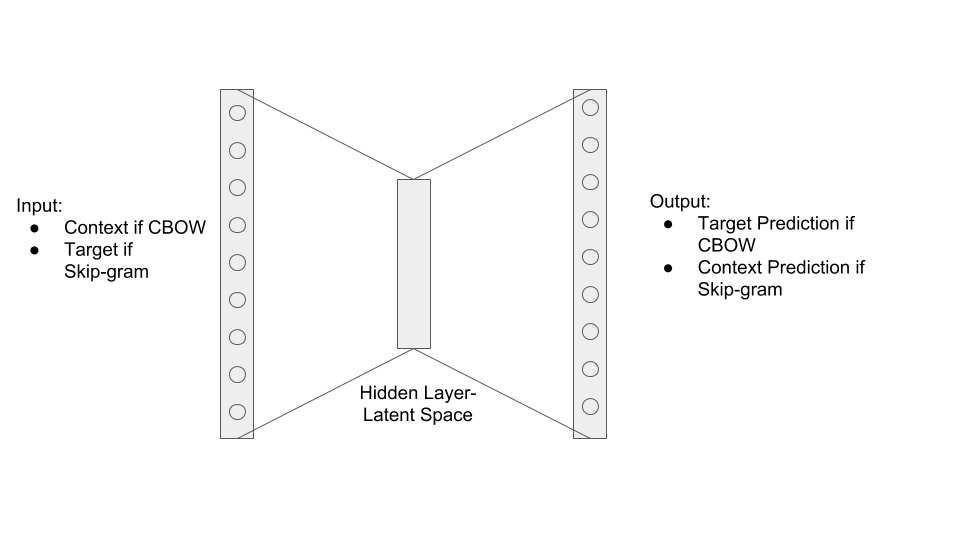
\includegraphics[width=0.45\textwidth]{images/nn_embedding_layer.png}
    \caption{Simple Embedding Layer Architecture}
    \label{fig:Embedding Layer Architecture}
\end{figure}
An embedding layer as part of a neural network is framed as the weights of the hidden layer in a single hidden layer dense feedforward neural network. Generally there are two ways of training such a model; by predicting the target object given that object's context as input (Continuous Bag of Words - CBOW) or by predicting the context of a target object given that object as input (Skip-gram).

\subsubsection{SVD Embedding Layers}
 \begin{figure}[h]
    \centering
    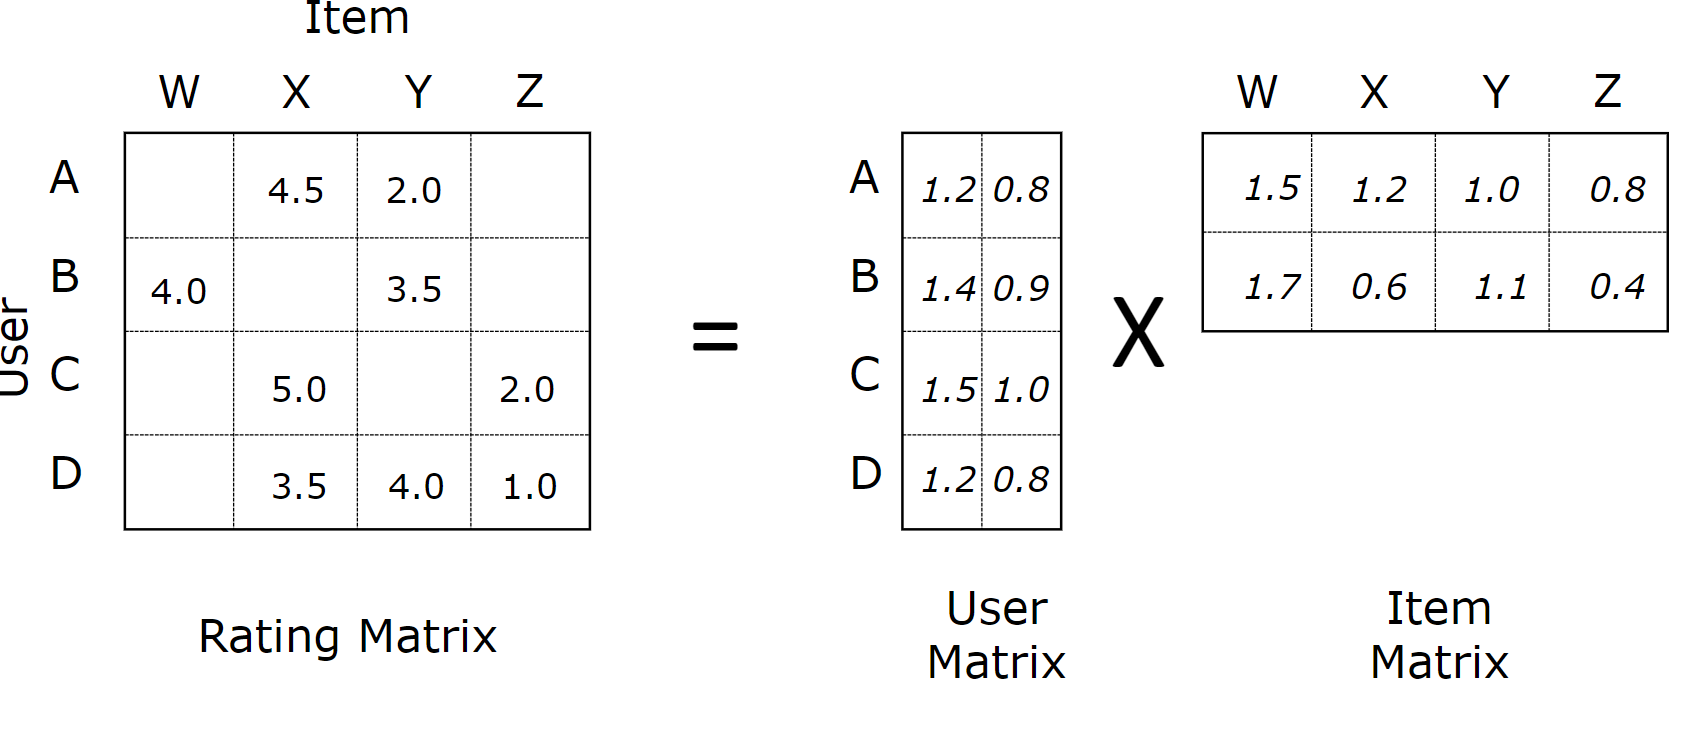
\includegraphics[width=0.45\textwidth]{images/matrix_factorization.png}
    \caption{MF diagram}
    \label{fig:MF diagram}
\end{figure}
Singual Value Decomposition is a form of Matrix Factorization popular in tradition recommendation systems. The idea is to start with a matrix $A$ where each entry represents an interaction. In the case of a User-movie embedding (here after refered to as user embedding), the rows of $A$ represent a user and the columns represent a movie. As you can see from figure~\ref{fig:MF diagram} Every entry is either the users rating of that movie, or zero. You then decompose your matrix to the product of three matrices $A = U\Sigma V^t$ $A$ is an $M \times N$ matrix $U$ is a $M \times M$ matrix $\Sigma$ is an $M \times N$ rectangular diagnal matrix and $V$ is a $N \times N$ unitary matrix. To get a reduced approximation of $A$ we simply decide how many $k$ features we want and keep the $k$ most important features of $\Sigma$. Multiplying $U\Sigma$ will result in $A$ of rank $k$. In tradtional recommendation systems the multipying the reduced rank $\Sigma$ with all three matrices would result in a new approximation of $A$ with values filled in from the reduced rank approximation. The predicted ratings are then looked up in the matrix for an item. For our use case we were only intrested in the reduced space representatoin of the matrix not transforming it back so we kept only $U\Sigma$